\documentclass[a4paper]{book}
\usepackage{makeidx}
\usepackage{natbib}
\usepackage{graphicx}
\usepackage{multicol}
\usepackage{float}
\usepackage{listings}
\usepackage{color}
\usepackage{ifthen}
\usepackage[table]{xcolor}
\usepackage{textcomp}
\usepackage{alltt}
\usepackage{ifpdf}
\ifpdf
\usepackage[pdftex,
            pagebackref=true,
            colorlinks=true,
            linkcolor=blue,
            unicode
           ]{hyperref}
\else
\usepackage[ps2pdf,
            pagebackref=true,
            colorlinks=true,
            linkcolor=blue,
            unicode
           ]{hyperref}
\usepackage{pspicture}
\fi
\usepackage[utf8]{inputenc}
\usepackage[T2A]{fontenc}
\usepackage[russian]{babel}

\usepackage{mathptmx}
\usepackage[scaled=.90]{helvet}
\usepackage{courier}
\usepackage{sectsty}
\usepackage[titles]{tocloft}
\usepackage{doxygen}
\lstset{language=C++,inputencoding=utf8,basicstyle=\footnotesize,breaklines=true,breakatwhitespace=true,tabsize=8,numbers=left }
\makeindex
\setcounter{tocdepth}{3}
\renewcommand{\footrulewidth}{0.4pt}
\renewcommand{\familydefault}{\sfdefault}
\hfuzz=15pt
\setlength{\emergencystretch}{15pt}
\hbadness=750
\tolerance=750
\begin{document}
\hypersetup{pageanchor=false,citecolor=blue}
\begin{titlepage}
\vspace*{7cm}
\begin{center}
{\Large \-Rragraph\-Pro\-Creator \\[1ex]\large 1.\-0.\-0 }\\
\vspace*{1cm}
{\large Создано системой Doxygen 1.7.6.1}\\
\vspace*{0.5cm}
{\small Вс 12 Янв 2014 18:37:54}\\
\end{center}
\end{titlepage}
\clearemptydoublepage
\pagenumbering{roman}
\tableofcontents
\clearemptydoublepage
\pagenumbering{arabic}
\hypersetup{pageanchor=true,citecolor=blue}
\chapter{Алфавитный указатель классов}
\section{Иерархия классов}
Иерархия классов.\begin{DoxyCompactList}
\item \contentsline{section}{\-Object\-Pro\-Creator}{\pageref{classObjectProCreator}}{}
\begin{DoxyCompactList}
\item \contentsline{section}{\-Curve\-Pro\-Creator}{\pageref{classCurveProCreator}}{}
\item \contentsline{section}{\-Group\-Pro\-Creator}{\pageref{classGroupProCreator}}{}
\item \contentsline{section}{\-Plot\-Pro\-Creator}{\pageref{classPlotProCreator}}{}
\end{DoxyCompactList}
\item \contentsline{section}{\-Rragraph\-Pro\-Creator}{\pageref{classRragraphProCreator}}{}
\end{DoxyCompactList}

\chapter{Алфавитный указатель классов}
\section{Классы}
Классы с их кратким описанием.\begin{DoxyCompactList}
\item\contentsline{section}{\hyperlink{classCurveProCreator}{\-Curve\-Pro\-Creator} }{\pageref{classCurveProCreator}}{}
\item\contentsline{section}{\hyperlink{classGroupProCreator}{\-Group\-Pro\-Creator} }{\pageref{classGroupProCreator}}{}
\item\contentsline{section}{\hyperlink{classObjectProCreator}{\-Object\-Pro\-Creator} }{\pageref{classObjectProCreator}}{}
\item\contentsline{section}{\hyperlink{classPlotProCreator}{\-Plot\-Pro\-Creator} }{\pageref{classPlotProCreator}}{}
\item\contentsline{section}{\hyperlink{classRragraphProCreator}{\-Rragraph\-Pro\-Creator} }{\pageref{classRragraphProCreator}}{}
\end{DoxyCompactList}

\chapter{Классы}
\hypertarget{classCurveProCreator}{\section{Класс \-Curve\-Pro\-Creator}
\label{classCurveProCreator}\index{\-Curve\-Pro\-Creator@{\-Curve\-Pro\-Creator}}
}


{\ttfamily \#include $<$\-Curve\-Pro\-Creator.\-h$>$}

Граф наследования\-:\-Curve\-Pro\-Creator\-:\begin{figure}[H]
\begin{center}
\leavevmode
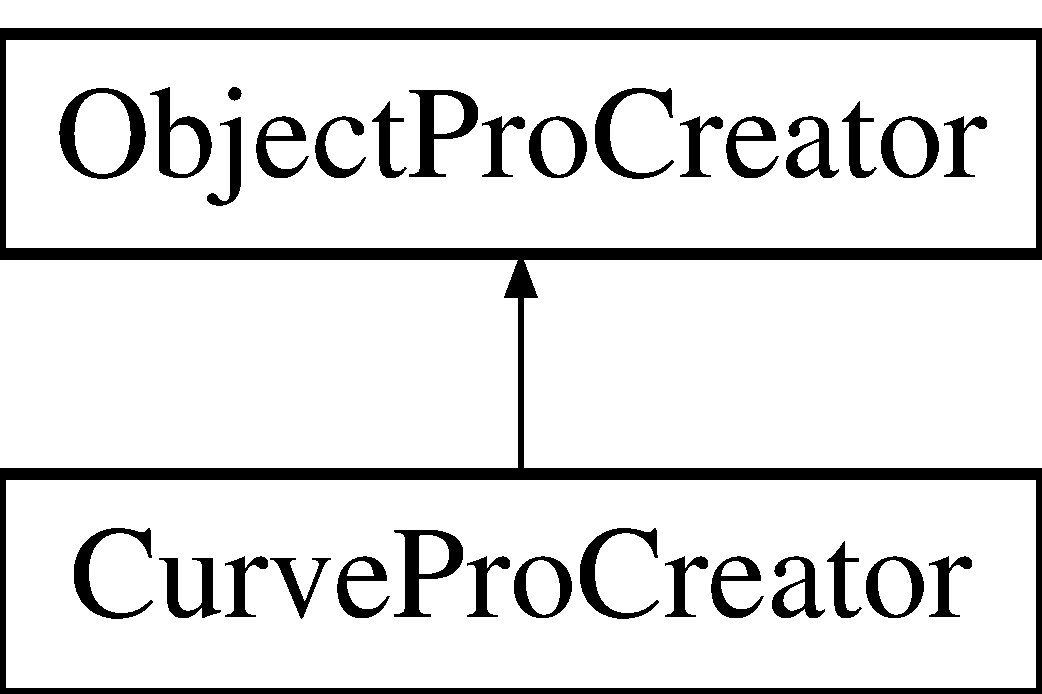
\includegraphics[height=2.000000cm]{classCurveProCreator}
\end{center}
\end{figure}
\subsection*{Открытые члены}
\begin{DoxyCompactItemize}
\item 
void \hyperlink{classCurveProCreator_a90b1f531a4059b8dc4ccbe5a9a17ef65}{set\-Color} (const \-Q\-String \&color)
\begin{DoxyCompactList}\small\item\em set\-Color -\/ Здесь задаётся цвет кривой. \end{DoxyCompactList}\item 
\hypertarget{classCurveProCreator_a61a75fe3cc91ae3a5b2cc92b7753930a}{void \hyperlink{classCurveProCreator_a61a75fe3cc91ae3a5b2cc92b7753930a}{set\-Width} (int width)}\label{classCurveProCreator_a61a75fe3cc91ae3a5b2cc92b7753930a}

\begin{DoxyCompactList}\small\item\em set\-Width -\/ Здесь задаётся ширина линии. \end{DoxyCompactList}\item 
void \hyperlink{classCurveProCreator_aa29b6611f233a0c3e42c513154c885af}{set\-Dash\-Pattern} (const \-Q\-String \&dash\-Pattern)
\begin{DoxyCompactList}\small\item\em set\-Dash\-Pattern -\/ Здесь задаётся штрих-\/пунктирная линия для кривой. Например если вы зададите строку \char`\"{}3 5 7 5\char`\"{}, кривая будет рисоваться следующим образом\-: штрих -\/ 3 px, пробел -\/ 5 px, штрих -\/ 7 px, пробел -\/ 5 px. \end{DoxyCompactList}\item 
void \hyperlink{classCurveProCreator_ae8e463e9680509d19c3d3de6c0bad98f}{set\-Symbol\-Style} (int style)
\begin{DoxyCompactList}\small\item\em set\-Symbol\-Style -\/ Установить фигуру, которая будет нарисована на точках кривой. \end{DoxyCompactList}\item 
\hypertarget{classCurveProCreator_a3be6f39528fb1906adc2e2c4f893b38a}{void \hyperlink{classCurveProCreator_a3be6f39528fb1906adc2e2c4f893b38a}{set\-Addend\-X} (double addend)}\label{classCurveProCreator_a3be6f39528fb1906adc2e2c4f893b38a}

\begin{DoxyCompactList}\small\item\em set\-Addend\-X -\/ Позволяет задать смещение кривой по оси \-X. \end{DoxyCompactList}\item 
\hypertarget{classCurveProCreator_afb25fc5c1691980a10bed6cd5d7dea2d}{void \hyperlink{classCurveProCreator_afb25fc5c1691980a10bed6cd5d7dea2d}{set\-Addend\-Y} (double addend)}\label{classCurveProCreator_afb25fc5c1691980a10bed6cd5d7dea2d}

\begin{DoxyCompactList}\small\item\em set\-Addend\-Y -\/ Позволяет задать смещение кривой по оси \-Y. \end{DoxyCompactList}\item 
\hypertarget{classCurveProCreator_a3881b8bbfddabf56538c58928347418f}{void \hyperlink{classCurveProCreator_a3881b8bbfddabf56538c58928347418f}{set\-Mult\-Y} (double addend)}\label{classCurveProCreator_a3881b8bbfddabf56538c58928347418f}

\begin{DoxyCompactList}\small\item\em set\-Mult\-Y -\/ Позволяет масштабировать кривую по оси \-Y. \end{DoxyCompactList}\item 
\hypertarget{classCurveProCreator_ad385e385cce634ab07c33a1cc6b9d0ba}{void \hyperlink{classCurveProCreator_ad385e385cce634ab07c33a1cc6b9d0ba}{set\-Step} (int step)}\label{classCurveProCreator_ad385e385cce634ab07c33a1cc6b9d0ba}

\begin{DoxyCompactList}\small\item\em Если кривая содержит много точек на количество пикселей и вы хотите раставить маркеры на кривой -\/ set\-Symbol\-Style(style != -\/1) -\/ тогда символы будут наезжать друг на друга. Чтобы этого избежать, задайте шаг для точек, на которых вы хотите рисовать символ. \end{DoxyCompactList}\item 
\hypertarget{classCurveProCreator_af512caf8250b70448d6587242b246d66}{void \hyperlink{classCurveProCreator_af512caf8250b70448d6587242b246d66}{set\-Y} (int i\-Y)}\label{classCurveProCreator_af512caf8250b70448d6587242b246d66}

\begin{DoxyCompactList}\small\item\em set\-Y -\/ Кривая имеет привязку к данным, загруженным из какого-\/то файла. Данный метод метод задаёт индекс столбца, который является \-Y -\/ составляющей кривой. \-X -\/ составляющая и сам файл задаётся в более высокой структуре. \end{DoxyCompactList}\end{DoxyCompactItemize}


\subsection{Подробное описание}
Класс предоставляет интерфейс для описания настроек кривой. 

\subsection{Методы}
\hypertarget{classCurveProCreator_a90b1f531a4059b8dc4ccbe5a9a17ef65}{\index{\-Curve\-Pro\-Creator@{\-Curve\-Pro\-Creator}!set\-Color@{set\-Color}}
\index{set\-Color@{set\-Color}!CurveProCreator@{\-Curve\-Pro\-Creator}}
\subsubsection[{set\-Color}]{\setlength{\rightskip}{0pt plus 5cm}void {\bf \-Curve\-Pro\-Creator\-::set\-Color} (
\begin{DoxyParamCaption}
\item[{const \-Q\-String \&}]{color}
\end{DoxyParamCaption}
)}}\label{classCurveProCreator_a90b1f531a4059b8dc4ccbe5a9a17ef65}


set\-Color -\/ Здесь задаётся цвет кривой. 


\begin{DoxyCode}
 CurveProCreator curve;
 curve.setColor("#ff0000")
\end{DoxyCode}
 \hypertarget{classCurveProCreator_aa29b6611f233a0c3e42c513154c885af}{\index{\-Curve\-Pro\-Creator@{\-Curve\-Pro\-Creator}!set\-Dash\-Pattern@{set\-Dash\-Pattern}}
\index{set\-Dash\-Pattern@{set\-Dash\-Pattern}!CurveProCreator@{\-Curve\-Pro\-Creator}}
\subsubsection[{set\-Dash\-Pattern}]{\setlength{\rightskip}{0pt plus 5cm}void {\bf \-Curve\-Pro\-Creator\-::set\-Dash\-Pattern} (
\begin{DoxyParamCaption}
\item[{const \-Q\-String \&}]{dash\-Pattern}
\end{DoxyParamCaption}
)}}\label{classCurveProCreator_aa29b6611f233a0c3e42c513154c885af}


set\-Dash\-Pattern -\/ Здесь задаётся штрих-\/пунктирная линия для кривой. Например если вы зададите строку \char`\"{}3 5 7 5\char`\"{}, кривая будет рисоваться следующим образом\-: штрих -\/ 3 px, пробел -\/ 5 px, штрих -\/ 7 px, пробел -\/ 5 px. 


\begin{DoxyParams}{Аргументы}
{\em dash\-Pattern} & \\
\hline
\end{DoxyParams}
\hypertarget{classCurveProCreator_ae8e463e9680509d19c3d3de6c0bad98f}{\index{\-Curve\-Pro\-Creator@{\-Curve\-Pro\-Creator}!set\-Symbol\-Style@{set\-Symbol\-Style}}
\index{set\-Symbol\-Style@{set\-Symbol\-Style}!CurveProCreator@{\-Curve\-Pro\-Creator}}
\subsubsection[{set\-Symbol\-Style}]{\setlength{\rightskip}{0pt plus 5cm}void {\bf \-Curve\-Pro\-Creator\-::set\-Symbol\-Style} (
\begin{DoxyParamCaption}
\item[{int}]{style}
\end{DoxyParamCaption}
)}}\label{classCurveProCreator_ae8e463e9680509d19c3d3de6c0bad98f}


set\-Symbol\-Style -\/ Установить фигуру, которая будет нарисована на точках кривой. 


\begin{DoxyParams}{Аргументы}
{\em style} & -\/ Указывает вид фигуры. Какая цифра какой фигуре соответствует смотрите в документации к библиотеке \-Qwt. \\
\hline
\end{DoxyParams}


Объявления и описания членов классов находятся в файлах\-:\begin{DoxyCompactItemize}
\item 
/home/rasmadeus/\-Documents/\-Projects/\-Q\-T/\-Rragraph/src/libs/\-Rragraph\-Pro\-Creator/\-Curve\-Pro\-Creator.\-h\item 
/home/rasmadeus/\-Documents/\-Projects/\-Q\-T/\-Rragraph/src/libs/\-Rragraph\-Pro\-Creator/\-Curve\-Pro\-Creator.\-cpp\end{DoxyCompactItemize}

\hypertarget{classGroupProCreator}{\section{Класс \-Group\-Pro\-Creator}
\label{classGroupProCreator}\index{\-Group\-Pro\-Creator@{\-Group\-Pro\-Creator}}
}
Граф наследования\-:\-Group\-Pro\-Creator\-:\begin{figure}[H]
\begin{center}
\leavevmode
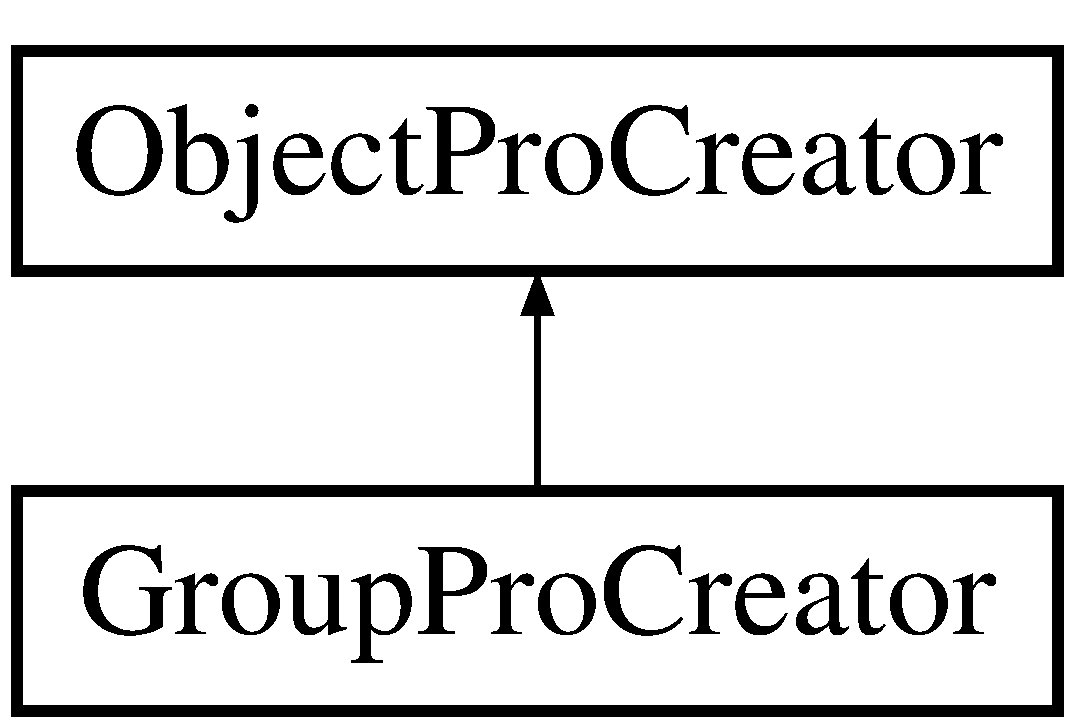
\includegraphics[height=2.000000cm]{classGroupProCreator}
\end{center}
\end{figure}
\subsection*{Открытые члены}
\begin{DoxyCompactItemize}
\item 
\hypertarget{classGroupProCreator_ac4f041a6f33e3e82ade28155617a7336}{void \hyperlink{classGroupProCreator_ac4f041a6f33e3e82ade28155617a7336}{clear} ()}\label{classGroupProCreator_ac4f041a6f33e3e82ade28155617a7336}

\begin{DoxyCompactList}\small\item\em clear -\/ Метод производит очистку экземпляра класса от всех внесённых изменений. Данная функция бывает полезна, например для того, чтобы сбросить ранее внесённые настройки и повторно использовать экземпляр класса. \end{DoxyCompactList}\item 
void \hyperlink{classGroupProCreator_add3e03e3b53e95959d1ed67092263dd7}{fill} (\-Q\-Json\-Array \&groups) const 
\begin{DoxyCompactList}\small\item\em fill -\/ Экземпляры данного класса и экземпляры его потомков рекомендуется использовать в качестве элемента коллекции \-Q\-Json\-Array. Данная функция добавляет текущий экземпляр в коллекцию. \end{DoxyCompactList}\item 
\hypertarget{classGroupProCreator_ae1766bbc8308f331d259383b90fac3c8}{void {\bfseries append\-File} (const \-Q\-String \&relative\-Path)}\label{classGroupProCreator_ae1766bbc8308f331d259383b90fac3c8}

\item 
\hypertarget{classGroupProCreator_acc072473508e5067f3173e1d0a1bd513}{void {\bfseries append\-Plot} (const \hyperlink{classPlotProCreator}{\-Plot\-Pro\-Creator} \&plot)}\label{classGroupProCreator_acc072473508e5067f3173e1d0a1bd513}

\item 
\hypertarget{classGroupProCreator_ab4bb6ed9b2f70bb8f9285f547d533fe5}{void {\bfseries append\-Curve} (const \-Curves\-Pro\-Creator \&curves)}\label{classGroupProCreator_ab4bb6ed9b2f70bb8f9285f547d533fe5}

\item 
\hypertarget{classGroupProCreator_a8527f79180870b91107bd3837b2fdc95}{void {\bfseries set\-Title} (const \-Q\-String \&title)}\label{classGroupProCreator_a8527f79180870b91107bd3837b2fdc95}

\end{DoxyCompactItemize}
\subsection*{Защищенные данные}
\begin{DoxyCompactItemize}
\item 
\hypertarget{classGroupProCreator_a163d86076fe89ee90b7058459184316d}{\-Q\-Json\-Array {\bfseries files}}\label{classGroupProCreator_a163d86076fe89ee90b7058459184316d}

\item 
\hypertarget{classGroupProCreator_a7efb6f7c19d8ef3ff7fd0070eac10789}{\-Q\-Json\-Array {\bfseries plots}}\label{classGroupProCreator_a7efb6f7c19d8ef3ff7fd0070eac10789}

\item 
\hypertarget{classGroupProCreator_a0fedff0994071612e7125db7fad157ca}{\-Q\-Json\-Array {\bfseries curves}}\label{classGroupProCreator_a0fedff0994071612e7125db7fad157ca}

\end{DoxyCompactItemize}


\subsection{Методы}
\hypertarget{classGroupProCreator_add3e03e3b53e95959d1ed67092263dd7}{\index{\-Group\-Pro\-Creator@{\-Group\-Pro\-Creator}!fill@{fill}}
\index{fill@{fill}!GroupProCreator@{\-Group\-Pro\-Creator}}
\subsubsection[{fill}]{\setlength{\rightskip}{0pt plus 5cm}void {\bf \-Group\-Pro\-Creator\-::fill} (
\begin{DoxyParamCaption}
\item[{\-Q\-Json\-Array \&}]{obj\-Array}
\end{DoxyParamCaption}
) const}}\label{classGroupProCreator_add3e03e3b53e95959d1ed67092263dd7}


fill -\/ Экземпляры данного класса и экземпляры его потомков рекомендуется использовать в качестве элемента коллекции \-Q\-Json\-Array. Данная функция добавляет текущий экземпляр в коллекцию. 


\begin{DoxyParams}{Аргументы}
{\em obj\-Array} & -\/ В данную коллекцию будет занесены настройки, содержащиеся в текущем экземпляре. \\
\hline
\end{DoxyParams}


Переопределяет метод предка \hyperlink{classObjectProCreator_ad207409ada5bbdef1dd4cf5e0d7d6f1d}{\-Object\-Pro\-Creator}.



Объявления и описания членов классов находятся в файлах\-:\begin{DoxyCompactItemize}
\item 
/home/rasmadeus/\-Documents/\-Projects/\-Q\-T/\-Rragraph/src/libs/\-Rragraph\-Pro\-Creator/\-Group\-Pro\-Creator.\-h\item 
/home/rasmadeus/\-Documents/\-Projects/\-Q\-T/\-Rragraph/src/libs/\-Rragraph\-Pro\-Creator/\-Group\-Pro\-Creator.\-cpp\end{DoxyCompactItemize}

\hypertarget{classObjectProCreator}{\section{Класс \-Object\-Pro\-Creator}
\label{classObjectProCreator}\index{\-Object\-Pro\-Creator@{\-Object\-Pro\-Creator}}
}


{\ttfamily \#include $<$\-Object\-Pro\-Creator.\-h$>$}

Граф наследования\-:\-Object\-Pro\-Creator\-:\begin{figure}[H]
\begin{center}
\leavevmode
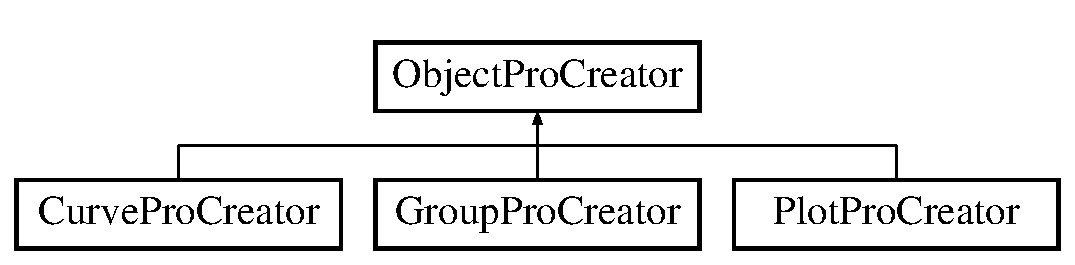
\includegraphics[height=2.000000cm]{classObjectProCreator}
\end{center}
\end{figure}
\subsection*{Открытые члены}
\begin{DoxyCompactItemize}
\item 
\hypertarget{classObjectProCreator_af975e9ddbd57c577bcab63b062a2da2b}{void \hyperlink{classObjectProCreator_af975e9ddbd57c577bcab63b062a2da2b}{clear} ()}\label{classObjectProCreator_af975e9ddbd57c577bcab63b062a2da2b}

\begin{DoxyCompactList}\small\item\em clear -\/ Метод производит очистку экземпляра класса от всех внесённых изменений. Данная функция бывает полезна, например для того, чтобы сбросить ранее внесённые настройки и повторно использовать экземпляр класса. \end{DoxyCompactList}\item 
void \hyperlink{classObjectProCreator_ad207409ada5bbdef1dd4cf5e0d7d6f1d}{fill} (\-Q\-Json\-Array \&obj\-Array) const 
\begin{DoxyCompactList}\small\item\em fill -\/ Экземпляры данного класса и экземпляры его потомков рекомендуется использовать в качестве элемента коллекции \-Q\-Json\-Array. Данная функция добавляет текущий экземпляр в коллекцию. \end{DoxyCompactList}\end{DoxyCompactItemize}
\subsection*{Защищенные члены}
\begin{DoxyCompactItemize}
\item 
void \hyperlink{classObjectProCreator_a5f00e7e6ef89bbe759da573071471460}{insert\-Property} (const \-Q\-String \&key, const \-Q\-Variant \&value)
\begin{DoxyCompactList}\small\item\em insert\-Property -\/ Метод добавляет к настройкам новое поле. \end{DoxyCompactList}\end{DoxyCompactItemize}
\subsection*{Защищенные данные}
\begin{DoxyCompactItemize}
\item 
\hypertarget{classObjectProCreator_a1682a1b31905120d46ab47eac40de074}{\-Q\-Json\-Object \hyperlink{classObjectProCreator_a1682a1b31905120d46ab47eac40de074}{obj}}\label{classObjectProCreator_a1682a1b31905120d46ab47eac40de074}

\begin{DoxyCompactList}\small\item\em obj -\/ Хранит текущие настройки. Объявлен как mutable, так как может изменяется из константной функции fill(...) const. \end{DoxyCompactList}\end{DoxyCompactItemize}


\subsection{Подробное описание}
Базовый класс для всех сущностей, которые необходимо описать в проектном файле. 

\subsection{Методы}
\hypertarget{classObjectProCreator_ad207409ada5bbdef1dd4cf5e0d7d6f1d}{\index{\-Object\-Pro\-Creator@{\-Object\-Pro\-Creator}!fill@{fill}}
\index{fill@{fill}!ObjectProCreator@{\-Object\-Pro\-Creator}}
\subsubsection[{fill}]{\setlength{\rightskip}{0pt plus 5cm}void {\bf \-Object\-Pro\-Creator\-::fill} (
\begin{DoxyParamCaption}
\item[{\-Q\-Json\-Array \&}]{obj\-Array}
\end{DoxyParamCaption}
) const}}\label{classObjectProCreator_ad207409ada5bbdef1dd4cf5e0d7d6f1d}


fill -\/ Экземпляры данного класса и экземпляры его потомков рекомендуется использовать в качестве элемента коллекции \-Q\-Json\-Array. Данная функция добавляет текущий экземпляр в коллекцию. 


\begin{DoxyParams}{Аргументы}
{\em obj\-Array} & -\/ В данную коллекцию будет занесены настройки, содержащиеся в текущем экземпляре. \\
\hline
\end{DoxyParams}


Переопределяется в \hyperlink{classGroupProCreator_add3e03e3b53e95959d1ed67092263dd7}{\-Group\-Pro\-Creator}.

\hypertarget{classObjectProCreator_a5f00e7e6ef89bbe759da573071471460}{\index{\-Object\-Pro\-Creator@{\-Object\-Pro\-Creator}!insert\-Property@{insert\-Property}}
\index{insert\-Property@{insert\-Property}!ObjectProCreator@{\-Object\-Pro\-Creator}}
\subsubsection[{insert\-Property}]{\setlength{\rightskip}{0pt plus 5cm}void {\bf \-Object\-Pro\-Creator\-::insert\-Property} (
\begin{DoxyParamCaption}
\item[{const \-Q\-String \&}]{key, }
\item[{const \-Q\-Variant \&}]{value}
\end{DoxyParamCaption}
)\hspace{0.3cm}{\ttfamily  \mbox{[}protected\mbox{]}}}}\label{classObjectProCreator_a5f00e7e6ef89bbe759da573071471460}


insert\-Property -\/ Метод добавляет к настройкам новое поле. 


\begin{DoxyParams}{Аргументы}
{\em key} & -\/ Ключ поля. \\
\hline
{\em value} & -\/ Значение поля. \\
\hline
\end{DoxyParams}


Объявления и описания членов классов находятся в файлах\-:\begin{DoxyCompactItemize}
\item 
/home/rasmadeus/\-Documents/\-Projects/\-Q\-T/\-Rragraph/src/libs/\-Rragraph\-Pro\-Creator/\-Object\-Pro\-Creator.\-h\item 
/home/rasmadeus/\-Documents/\-Projects/\-Q\-T/\-Rragraph/src/libs/\-Rragraph\-Pro\-Creator/\-Object\-Pro\-Creator.\-cpp\end{DoxyCompactItemize}

\hypertarget{classPlotProCreator}{\section{Класс \-Plot\-Pro\-Creator}
\label{classPlotProCreator}\index{\-Plot\-Pro\-Creator@{\-Plot\-Pro\-Creator}}
}
Граф наследования\-:\-Plot\-Pro\-Creator\-:\begin{figure}[H]
\begin{center}
\leavevmode
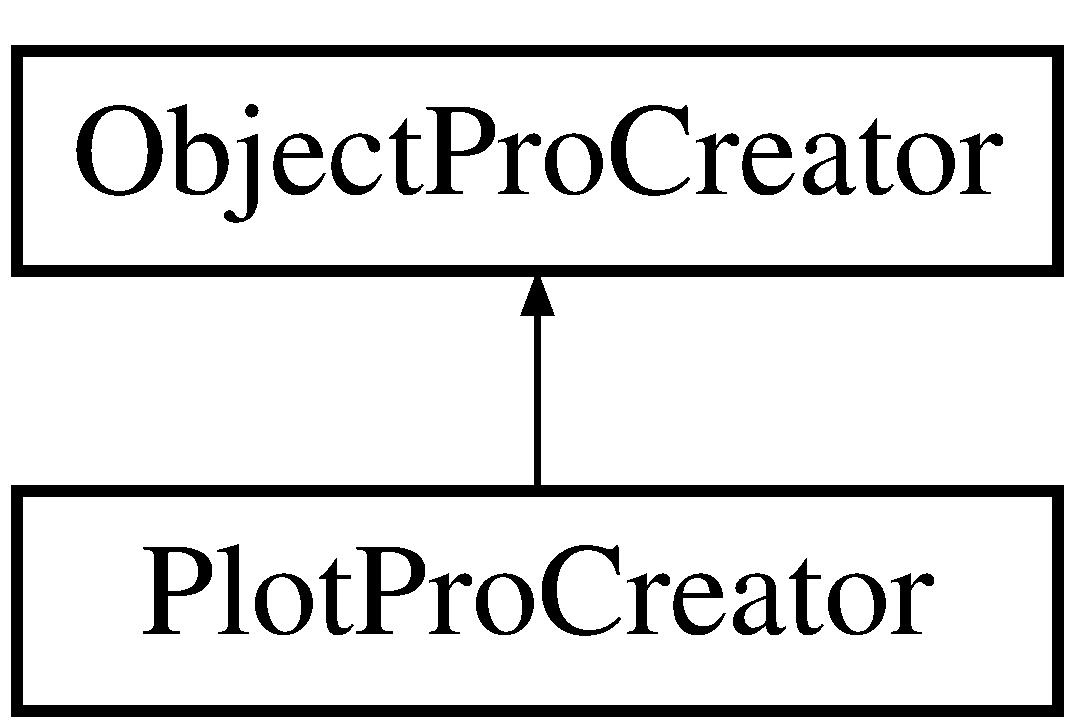
\includegraphics[height=2.000000cm]{classPlotProCreator}
\end{center}
\end{figure}
\subsection*{Открытые члены}
\begin{DoxyCompactItemize}
\item 
\hypertarget{classPlotProCreator_ab314b6a6b180c598d1b64e5c5c4d7a70}{void {\bfseries set\-Title} (const \-Q\-String \&title)}\label{classPlotProCreator_ab314b6a6b180c598d1b64e5c5c4d7a70}

\item 
\hypertarget{classPlotProCreator_abae4f2c2ffe78d3c5ddf5d67a35af6aa}{void {\bfseries set\-X\-Title} (const \-Q\-String \&title)}\label{classPlotProCreator_abae4f2c2ffe78d3c5ddf5d67a35af6aa}

\item 
\hypertarget{classPlotProCreator_aa44ab8fb1b26f8ae88c4053a22692301}{void {\bfseries set\-Y\-Title} (const \-Q\-String \&title)}\label{classPlotProCreator_aa44ab8fb1b26f8ae88c4053a22692301}

\item 
\hypertarget{classPlotProCreator_a6df2c1f23d486f06fe5f41f316ed33c5}{void {\bfseries set\-Rect} (const \-Q\-Rect\-F \&rect)}\label{classPlotProCreator_a6df2c1f23d486f06fe5f41f316ed33c5}

\item 
\hypertarget{classPlotProCreator_a84522e991e8465ba8dce3084eac02ddc}{void {\bfseries set\-Steps} (const \-Q\-Point\-F \&steps)}\label{classPlotProCreator_a84522e991e8465ba8dce3084eac02ddc}

\item 
\hypertarget{classPlotProCreator_a9ac8966ef4f9753ef4da56e55c6f812b}{void {\bfseries set\-Export\-Size} (const \-Q\-Size\-F \&size)}\label{classPlotProCreator_a9ac8966ef4f9753ef4da56e55c6f812b}

\item 
\hypertarget{classPlotProCreator_aabbac7119f882dd12d5efc06d3e3a7f8}{void {\bfseries set\-Legend\-Opacity} (int opacity)}\label{classPlotProCreator_aabbac7119f882dd12d5efc06d3e3a7f8}

\item 
\hypertarget{classPlotProCreator_aac9f94da42427bc4b1f121679fc1142a}{void {\bfseries set\-Legend\-Position} (int hor\-Pos, int ver\-Pos)}\label{classPlotProCreator_aac9f94da42427bc4b1f121679fc1142a}

\end{DoxyCompactItemize}


Объявления и описания членов классов находятся в файлах\-:\begin{DoxyCompactItemize}
\item 
/home/rasmadeus/\-Documents/\-Projects/\-Q\-T/\-Rragraph/src/libs/\-Rragraph\-Pro\-Creator/\-Plot\-Pro\-Creator.\-h\item 
/home/rasmadeus/\-Documents/\-Projects/\-Q\-T/\-Rragraph/src/libs/\-Rragraph\-Pro\-Creator/\-Plot\-Pro\-Creator.\-cpp\end{DoxyCompactItemize}

\hypertarget{classRragraphProCreator}{\section{Класс \-Rragraph\-Pro\-Creator}
\label{classRragraphProCreator}\index{\-Rragraph\-Pro\-Creator@{\-Rragraph\-Pro\-Creator}}
}
\subsection*{Открытые члены}
\begin{DoxyCompactItemize}
\item 
bool \hyperlink{classRragraphProCreator_ab90070ea892bb8088a06ec54ab89f13a}{read} (const \-Q\-String \&path\-To\-Pro)
\begin{DoxyCompactList}\small\item\em read -\/ Метод предназначен для чтения проектного файла программы \-Rragraph с жёсткого диска или другого носителя. Все внесённые изменения в объект до вызова этого метода будут потеряны. \end{DoxyCompactList}\item 
bool \hyperlink{classRragraphProCreator_a0b6c0794de85961a1f0643ec23e8e092}{save} (const \-Q\-String \&path\-To\-Pro) const 
\begin{DoxyCompactList}\small\item\em save -\/ Метод предназначен для сохранения проектного файла программы \-Rragraph на жёсткий диск или на иной носитель. \end{DoxyCompactList}\item 
\hypertarget{classRragraphProCreator_ac259b4d4ebdd44477442126743207a5f}{void \hyperlink{classRragraphProCreator_ac259b4d4ebdd44477442126743207a5f}{clear} ()}\label{classRragraphProCreator_ac259b4d4ebdd44477442126743207a5f}

\begin{DoxyCompactList}\small\item\em clear -\/ Данный метод очищает объект от всех ранее внесённых изменений. \end{DoxyCompactList}\item 
\hypertarget{classRragraphProCreator_a10c0c0fcd520eae2dcdda77367a53334}{void \hyperlink{classRragraphProCreator_a10c0c0fcd520eae2dcdda77367a53334}{append\-Group} (\hyperlink{classGroupProCreator}{\-Group\-Pro\-Creator} \&group)}\label{classRragraphProCreator_a10c0c0fcd520eae2dcdda77367a53334}

\begin{DoxyCompactList}\small\item\em append\-Group -\/ Метод создаёт новую группу графиков. \end{DoxyCompactList}\end{DoxyCompactItemize}
\subsection*{Защищенные данные}
\begin{DoxyCompactItemize}
\item 
\hypertarget{classRragraphProCreator_a5143a23f647648ed25f3f2bb206226bf}{\-Q\-Json\-Array \hyperlink{classRragraphProCreator_a5143a23f647648ed25f3f2bb206226bf}{groups}}\label{classRragraphProCreator_a5143a23f647648ed25f3f2bb206226bf}

\begin{DoxyCompactList}\small\item\em groups -\/ Содержит описание групп графиков. \end{DoxyCompactList}\end{DoxyCompactItemize}


\subsection{Методы}
\hypertarget{classRragraphProCreator_ab90070ea892bb8088a06ec54ab89f13a}{\index{\-Rragraph\-Pro\-Creator@{\-Rragraph\-Pro\-Creator}!read@{read}}
\index{read@{read}!RragraphProCreator@{\-Rragraph\-Pro\-Creator}}
\subsubsection[{read}]{\setlength{\rightskip}{0pt plus 5cm}bool {\bf \-Rragraph\-Pro\-Creator\-::read} (
\begin{DoxyParamCaption}
\item[{const \-Q\-String \&}]{path\-To\-Pro}
\end{DoxyParamCaption}
)}}\label{classRragraphProCreator_ab90070ea892bb8088a06ec54ab89f13a}


read -\/ Метод предназначен для чтения проектного файла программы \-Rragraph с жёсткого диска или другого носителя. Все внесённые изменения в объект до вызова этого метода будут потеряны. 


\begin{DoxyParams}{Аргументы}
{\em path\-To\-Pro} & -\/ Путь к проектному файлу. \\
\hline
\end{DoxyParams}
\begin{DoxyReturn}{Возвращает}
-\/ Успешность чтения проектного файла. 
\end{DoxyReturn}
\hypertarget{classRragraphProCreator_a0b6c0794de85961a1f0643ec23e8e092}{\index{\-Rragraph\-Pro\-Creator@{\-Rragraph\-Pro\-Creator}!save@{save}}
\index{save@{save}!RragraphProCreator@{\-Rragraph\-Pro\-Creator}}
\subsubsection[{save}]{\setlength{\rightskip}{0pt plus 5cm}bool {\bf \-Rragraph\-Pro\-Creator\-::save} (
\begin{DoxyParamCaption}
\item[{const \-Q\-String \&}]{path\-To\-Pro}
\end{DoxyParamCaption}
) const}}\label{classRragraphProCreator_a0b6c0794de85961a1f0643ec23e8e092}


save -\/ Метод предназначен для сохранения проектного файла программы \-Rragraph на жёсткий диск или на иной носитель. 


\begin{DoxyParams}{Аргументы}
{\em path\-To\-Pro} & -\/ По данному пути будет сохранён проектный файл. \\
\hline
\end{DoxyParams}
\begin{DoxyReturn}{Возвращает}
-\/ Возвращает успешность сохранения проектного файла. 
\end{DoxyReturn}


Объявления и описания членов классов находятся в файлах\-:\begin{DoxyCompactItemize}
\item 
/home/rasmadeus/\-Documents/\-Projects/\-Q\-T/\-Rragraph/src/libs/\-Rragraph\-Pro\-Creator/\-Rragraph\-Pro\-Creator.\-h\item 
/home/rasmadeus/\-Documents/\-Projects/\-Q\-T/\-Rragraph/src/libs/\-Rragraph\-Pro\-Creator/\-Rragraph\-Pro\-Creator.\-cpp\end{DoxyCompactItemize}

\printindex
\end{document}
